\documentclass{article}
\usepackage[utf8]{inputenc}

\title{TT3010 - Audio technology and room acoustics. \newline Exercise 2 - Room acoustics \newline Solutions}
\author{Jan Arne Bosnes}
\date{\today}

\usepackage{natbib}
\usepackage{graphicx}
\usepackage{float}
\usepackage{gensymb}

\begin{document}

\maketitle

\section*{1}

The resonance frequencies of the room modes, or standing waves, in a shoebox-shaped room are:

\begin{equation}
    f_{lmn} = \frac{c}{2}\sqrt{\left(\frac{l}{l}\right)^2+\left(\frac{m}{w}\right)^2+\left(\frac{n}{h}\right)^2}
\end{equation}
where c is the speed of sound and l, m and n are integers.

To find the lowest resonance frequencies, we have to insert combinations of the lowest integers (0,1,2), for the room with length, $l=5m$, width, $w=10m$ and height $h=2.5m$ and get the following frequencies:

\begin{equation}
    f_{100} = \frac{c}{2}\sqrt{\left(\frac{1}{l}\right)^2+\left(\frac{0}{w}\right)^2+\left(\frac{0}{h}\right)^2} = 34.4 Hz
\end{equation}

\begin{equation}
    f_{010} = \frac{c}{2}\sqrt{\left(\frac{0}{l}\right)^2+\left(\frac{1}{w}\right)^2+\left(\frac{0}{h}\right)^2} = 17.2 Hz
\end{equation}

\begin{equation}
    f_{001} = \frac{c}{2}\sqrt{\left(\frac{0}{l}\right)^2+\left(\frac{0}{w}\right)^2+\left(\frac{1}{h}\right)^2} = 68.8 Hz
\end{equation}

\begin{equation}
    f_{020} = \frac{c}{2}\sqrt{\left(\frac{0}{l}\right)^2+\left(\frac{2}{w}\right)^2+\left(\frac{0}{h}\right)^2} = 34.4 Hz
\end{equation}

\begin{equation}
    f_{110} = \frac{c}{2}\sqrt{\left(\frac{1}{l}\right)^2+\left(\frac{1}{w}\right)^2+\left(\frac{0}{h}\right)^2} = 38.5 Hz
\end{equation}
etc

Apparantly, the three lowest ones are 17.2 Hz, 34.4 Hz, and 38.5 Hz, but the one at 17.2 Hz would have little influence in the audible range.

Around the resonance frequencies, the sound in the room will get particularly loud (if the source is emitting energy in that frequency range), but the variation of the sound level inside the room will also be much stronger (than in other frequency ranges).


%The modes help us understand the distribution of pressure in the room. Modes where two of the integers are zero and the other integer is nonzero, are called axial modes, because they consist of standing waves propagating back and forth between two parallel surfaces. In general, they inherit more acoustic energy because the sound travel farther between reflections. Modes where only one of the integers are nonzero are called tangential modes, which means that they travel on between four surfaces. They have lower acoustic energy than axial modes, but higher energy than oblique modes where all the integers are nonzero. This means that the modes uses all the walls in the room (4 surfaces) including the ceiling and the floor. So 6 surfaces in total. 


\section*{2}

The so-called hall radius can be found in two ways: either from the chart in Figure 1, or from the expression:

\begin{equation}
    L_p = L_w + 10 \log(\frac{Q}{4 \pi r^2}+\frac{4}{A})
\end{equation}
where $r$ is the distance, $Q$ is the directivity factor of the sound source, $A$ is the total absorption, $L_p$ is the sound pressure level at the listener/receiver and $L_W$ is the sound power level.

Method 1:

The chart shows how $L_p - L_W$ varies with distance, for various values of $A$. All curves flatten out for large values of distance (to the right) and as the hint says, we should look for a point where the curve is 3 dB higher than the flat part. In this task, $A=500$, so the flat part of the curve is at -21.7 dB. Using a ruler, one can find the point on the "500"-curve which is at -18.7 dB (3 dB higher than the flat area), and that happens at $r/\sqrt{Q} \approx 3.1$, see the drawing below. Since $Q$ was given to be 5, we find,
\[
r \approx \sqrt{Q} \cdot 3.1  = \sqrt{5} \cdot 3.1 \approx 6.9 m
\]

Method 2:
In the expression for $L_p$, the two terms for the direct sound and reverberation are equal when $r$ equals the room radius

\begin{equation}
    \frac{Q}{4\pi r^2} = \frac{4}{A}
\end{equation}

which can be rewritten:

\begin{equation}
 r = \sqrt{\frac{Q A}{16 \pi}} = \sqrt{\frac{5 \cdot 500}{16 \cdot \pi}} \approx 7m 
\end{equation}

%We can check this by calculating the 

%If one uses the hint that is given, we know that $L_p-L_w$. One may start by calculating the reverberant sound level:

%\begin{equation}
%    L_{p,reverberant} = L_w + 10 \log (\frac{4}{A}) \approx 21.7 dB
%\end{equation}

%and then calculate the direct sound:
%\begin{equation}
%    L_{p,direct} = L_w + 10 \log(\frac{Q}{4 \pi r^2}) \approx 17.9 dB
%\end{equation}

%then use the figure 1. to make sure that one is correct with the calculations that have been made.

\begin{figure}[H]
    \centering
    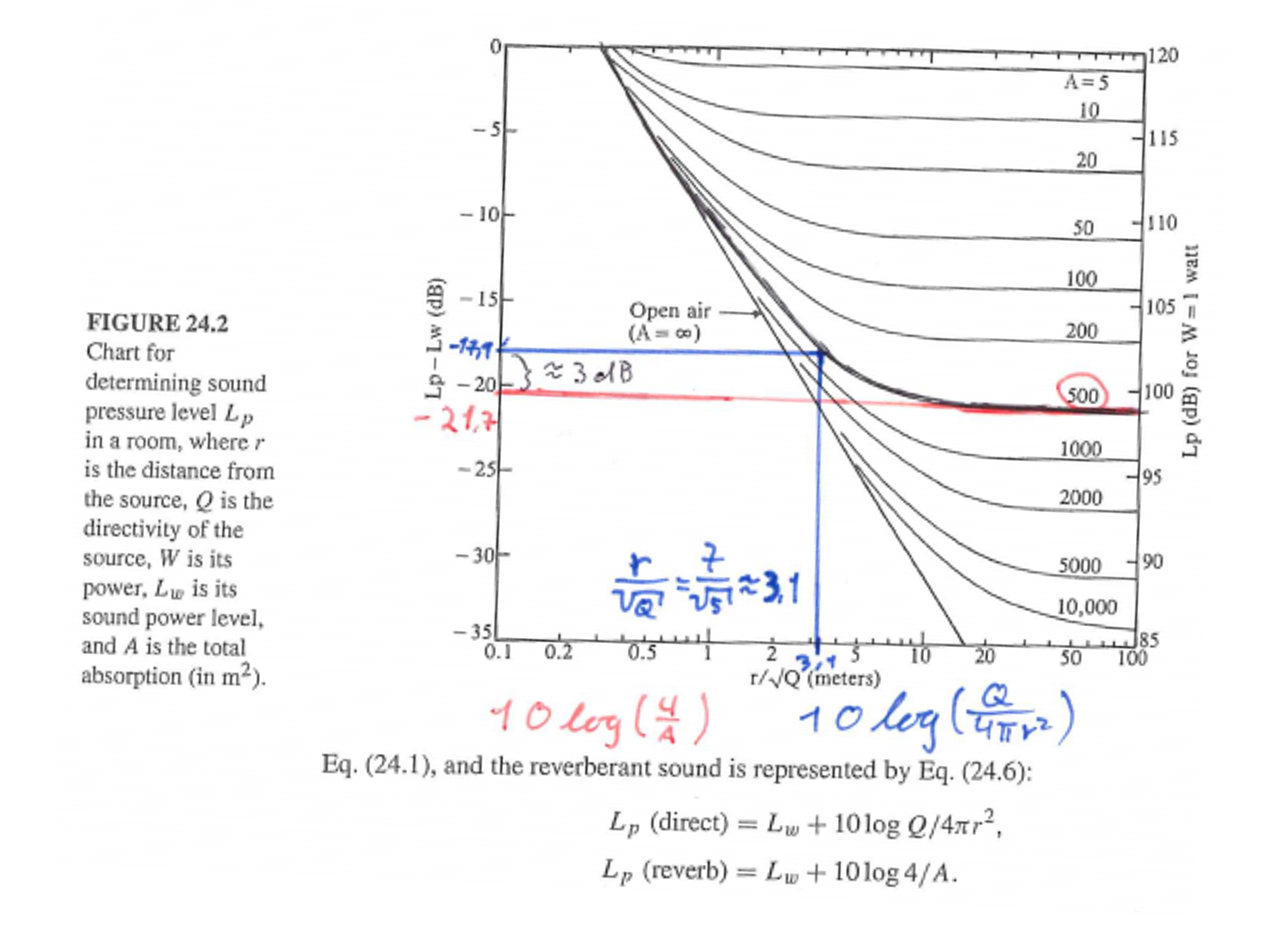
\includegraphics{figures/oving2_1_solution.png}
    \caption{My attempt on drawing of the direct sound (blue) and the reverberant sound (red).}
    \label{fig:my_label}
\end{figure}


\section*{3}
The sound pressure distribution for one room mode, or standing wave, can be illustrated by drawing vertical and horizontal lines, which illustrate so-called nodal lines, or zeroes. These are lines where it is very close to silent. 

The pressure of the axial modes are at its maxima on the walls itself. For a tangential mode, the maxima is in the center of the room as well as on the walls. Figure \ref{fig:1}, \ref{fig:2} and \ref{fig:3} shows the areas where the pressures are distributed.
\begin{figure}[H]
    \centering
    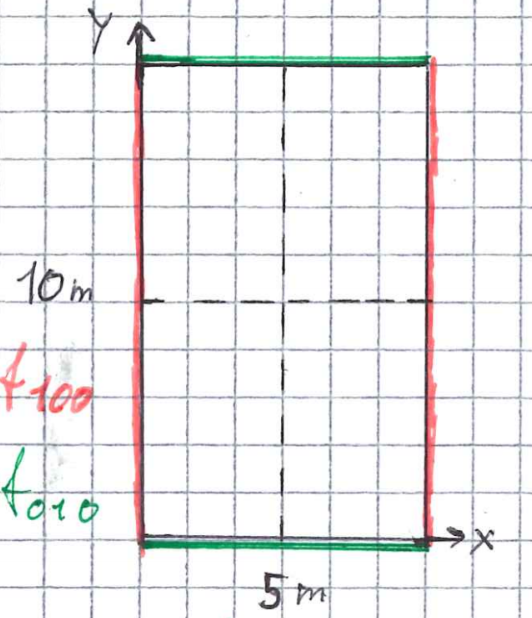
\includegraphics{figures/oving2_3_solution.png}
    \caption{Axial modes with max pressure at the walls. Dashed lines are node points.}
    \label{fig:1}
\end{figure}

\begin{figure}[H]
    \centering
    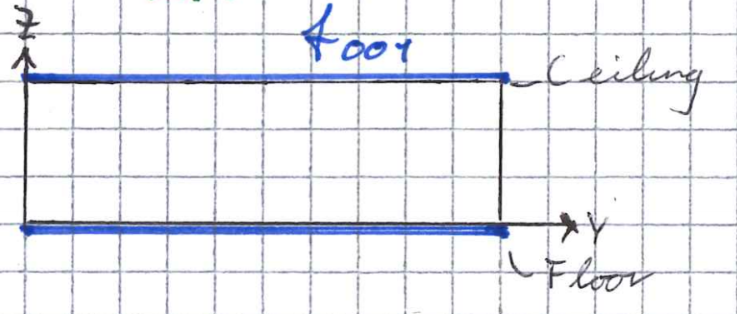
\includegraphics{figures/oving2_4_solution.png}
    \caption{Axial mode with max pressure at the roof an ceiling.}
    \label{fig:2}
\end{figure}

\begin{figure}[H]
    \centering
    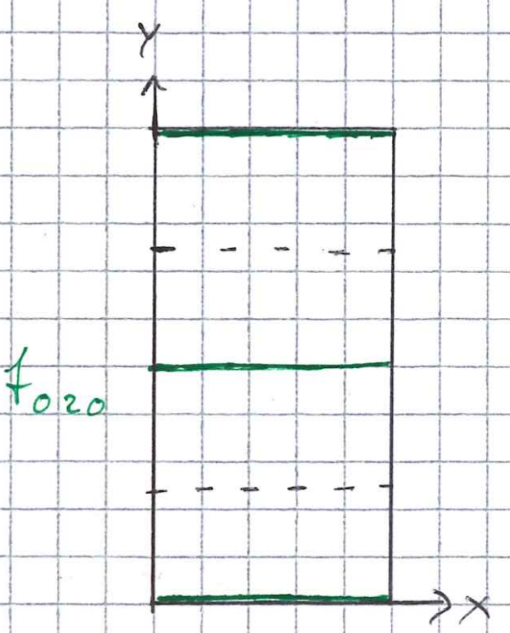
\includegraphics{figures/oving2_5_solution.png}
    \caption{Tangential modes with max pressure at the walls and in the center. Dashed lines are node points.}
    \label{fig:3}
\end{figure}

\begin{figure}
    \centering
    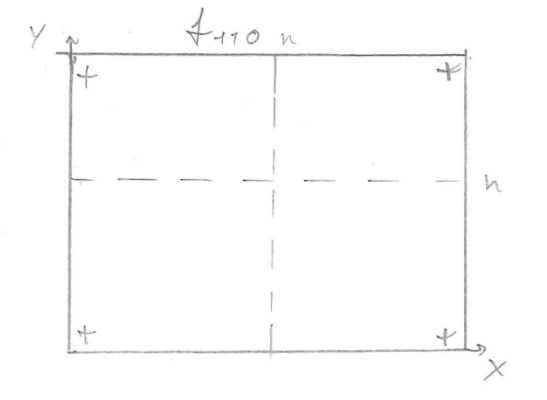
\includegraphics{figures/oving2_8_solution.png}
    \caption{Axial modes on the xy plane for frequency $f_{110}$}
    \label{fig:4}
\end{figure}

The pressure distribution for modes $f_{100}$, $f_{010}$ and $f_{001}$ will be as follows.

\begin{figure}[H]
    \centering
    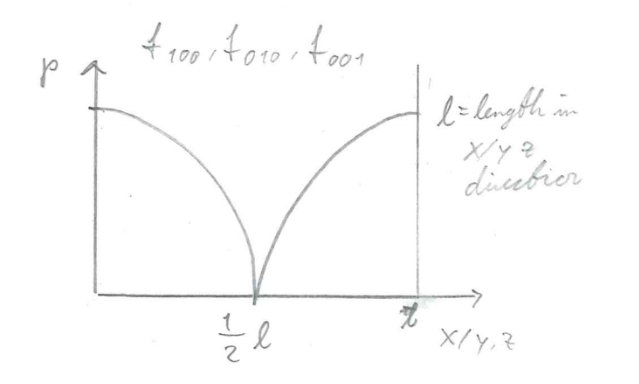
\includegraphics{figures/oving2_6_solution.png}
    \end{figure}

The pressure distribution for modes $f_{020}$ will be as follows.

\begin{figure}[H]
    \centering
    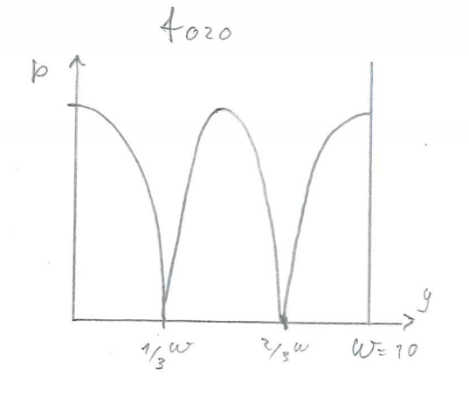
\includegraphics{figures/oving2_7_solution.png}
\end{figure}


\end{document}
